\clearpage

\chapter{A SICStus \clpb könyvtára}

A következő fejezetben a SICStus \clpb könyvtárával fogunk foglalkozni.
A \clpb könyvtárat az alábbi módon lehet használatba venni:
\begin{minted}{prolog}
:- use_module(library(clpb)).
\end{minted}

\section{A \clpb könyvtár általános jellemzése}

A \clpb könyvtár a kétértékű Boole-logikán alapuló CLP rendszert valósít meg,
ennek megfelelően a \clpb változók értékkészlete a ${0,1}$ halmaz.

\enumhead{Felhasználható függvények (egyben korlát-relációk)}
\btab{lp{30em}}
\cd{{\~{}} P}      &  \cd{P} hamis ({\it negáció}).\\
\cd{P * Q}     &  \cd{P} és \cd{Q} mindegyike igaz ({\it konjunkció}).\\
\cd{P + Q}     &  \cd{P} és \cd{Q} legalább egyike igaz ({\it
diszjunkció}).\\
\cd{P \# Q}    &  \cd{P} és \cd{Q} pontosan egyike igaz ({\it kizáró
vagy}).\\
\cd{X {\^{}} P}  &  Létezik olyan \cd{X}, hogy \cd{P} igaz (azaz \cd{P[X/0]+P[X/1]} igaz).\\
\verb'P =\= Q'  &  Ugyanaz, mint \verb'P # Q'.\\
\verb'P =:= Q'  &  Ugyanaz, mint \verb'~(P # Q)'.\\
\verb'P =< Q'   &  Ugyanaz, mint \verb'~P + Q'.\\
\verb'P >= Q'   &  Ugyanaz, mint \verb'P + ~Q'.\\
\verb'P < Q'    &  Ugyanaz, mint \verb'~P * Q'.\\
\verb'P > Q'    &  Ugyanaz, mint \verb'P * ~Q'.\\
\cd{card(Is, Es)} &  Az \cd{Es} listában szereplő igaz értékű
kifejezések száma eleme az \cd{Is} által jelölt halmaznak (\cd{Is}
egészek és \cd{Tol-Ig} szakaszok listája).\\
\etab

A \Clpb -ben az összes korlát egyszerű korlát, nincsenek összetett korlátok.
Pont ez a tény az, ami a \Clpb -t nagy feladatok megoldására alkalmatlanná
teszi, hiszen minden korlát azonnal bekerül a korlát-tárba, és egy idő után
a megoldó algoritmus (a Boole-egyesítés) működése a korlát-tár nagy mérete
miatt lelassul.

\enum{Alapvető könyvtári eljárások}{
\item \cd{sat(Kifejezés)} -- hozzáveszi \cd{Kifejezés}t a korlát-tárhoz.
\cd{Kifejezés} a \cd{0} és \cd{1} konstansokból, atomokból, valamint
változókból a fenti műveletekkel felépített logikai kifejezés. A kifejezésben
előforduló atomok a kifejezés legkülső szintjén univerzálisan kvantifikált
változókat jelentenek.

\item \cd{taut(Kifejezés,Érték)} -- megvizsgálja, hogy \cd{Kifejezés}
levezethető-e a korlát-tárból. Ha levezethető, akkor \cd{Érték}et \cd{1}-gyel
egyesíti. Ha \cd{Kifejezés} tagadása levezethető, akkor \cd{Érték}et \cd{0}-val
egyesíti. Minden más esetben meghiúsul.

\item \cd{labeling(Változók)} -- beállítja a \cd{Változók} lista összes
elemét 1-re vagy 0-ra úgy, hogy a korlát-tár teljesüljön. Visszalépésre az
összes lehetséges megoldást felsorolja.
}

\section{Példafutások a \clpb könyvtár segítségével}

\begin{minted}{prolog}
| ?- sat(X + Y).
sat(X=\=_A*Y#Y) ? 

| ?- sat(x + Y).
sat(Y=\=_A*x#x) ? 

| ?- taut(_A ^ (X=\=_A*Y#Y) =:= X+Y, T).
T = 1 ? 

| ?- sat(A # B =:= 0).
B = A ? 

| ?- sat(A # B =:= C), A = B.
B = A, C = 0 ? 

| ?- taut(A =< C, T).
no

| ?- sat(A =< B), sat(B =< C), taut(A =< C, T).
T = 1, sat(A=:=_A*_B*C), sat(B=:=_B*C) ? 
\end{minted}

Látható, hogy a \clpb a korlát-tár tartalmát \cd{sat(Kifejezés)} alakú
struktúrák konjunkciójaként jeleníti meg, ahol \cd{Kifejezés} mindig egy
,,polinom'', azaz konjunkciók kizáró vagy (\cd{\#}) műveletekkel képzett
sorozata. Az atomok a fent elmondottak szerint univerzálisan kvantifikált
változókat jelentenek. Az univerzális és az egzisztenciális kvantifikáció
különbségének kiemelésére nézzük meg az alábbi példákat is:

\begin{alltt}
| ?- sat(~x+ ~y=:= ~(x*y)).   % \(\forall\cd{xy}(\lnot\cd{x}\lor\lnot\cd{y}=\lnot(\cd{x}\land\cd{y}))\)
yes
| ?- sat(~X+ ~Y=:= ~(X*Y)).   % \(\exists?\cd{XY}(\lnot\cd{X}\lor\lnot\cd{Y}=\lnot(\cd{X}\land\cd{Y}))\)
true ? ; no
| ?- sat(x=<y).               % \(\forall\cd{xy}(\cd{x} \to \cd{y})\)
no
| ?- sat(X=<y).               % \(\forall\cd{y}\exists?\cd{X}(\cd{X} \to \cd{y})\) 
sat(X=:=_A*y) ? ; no
\end{alltt}

Nézzünk most egy picit komplikáltabb \clpb példát, amely egy egy bites
összeadó áramkör működését próbálja modellezni \clpb korlátok segítségével:

\begin{minted}{prolog}
| ?- [user].
| adder(X, Y, Sum, Cin, Cout) :-
     sat(Sum =:= card([1,3],[X,Y,Cin])),
     sat(Cout =:= card([2-3],[X,Y,Cin])).
| {user consulted, 40 msec 576 bytes}
yes
\end{minted}

Az összeadó működése a \cd{card/2} segítségével nagyon egyszerűen leírható:
az összeg értéke akkor 1, ha az \cd{[X,Y,Cin]} listában (\cd{Cin} a carry in,
tehát a bemenő átvitel rövidítése) 1 vagy 3 db egyes van, \cd{Cout}
(a kimenő átvitel) értéke pedig akkor 1, ha az \cd{[X,Y,Cin]} listában legalább
két db egyes van. Nézzük meg, hogy ezeket a korlátokat milyen formában tárolja
a \clpb rendszer!

\begin{minted}{prolog}
| ?- adder(x, y, Sum, cin, Cout).
sat(Sum=:=cin#x#y),
sat(Cout=:=x*cin#x*y#y*cin) ?
\end{minted}

Látható, hogy a \cd{card/2} itt is konjunkciók kizáró vagy kapcsolatára
vezetődött vissza. Mivel csak a \cd{Sum} és \cd{Cout} változók viselkedésére
voltunk kíváncsiak, ezért a másik három változót egzisztenciálisan
kvantifikáltuk. Nézzük meg azt az egyszerűsített esetet is, amikor \cd{Cin}-t
0-ra kötjük, tehát nincs bemenő átvitel:

\begin{minted}{prolog}
| ?- adder(x, y, Sum, 0, Cout).
sat(Sum=:=x#y),
sat(Cout=:=x*y) ?
\end{minted}

Ha a megoldás nem egyértelmű, akkor a \cd{labeling} eljárással tudjuk
felsoroltatni az összes lehetséges megoldást:

\begin{minted}{prolog}
| ?- adder(X, Y, 0, Cin, 1), labeling([X,Y,Cin]).
Cin = 0, X = 1, Y = 1 ? ; 
Cin = 1, X = 0, Y = 1 ? ;
Cin = 1, X = 1, Y = 0 ? ;
no
\end{minted}

\section{A Boole-egyesítés}

A \clpb könyvtár két Boole-kifejezés egyesítésére ,,meglepő módon'' a
Boole-egyesítés nevű algoritmust használja. A feladat pontos megfogalmazása:
legyen adott a $g$ és $h$ Boole-kifejezés, és keressük a $g = h$
egyenletet megoldó legáltalánosabb egyesítőt (a továbbiakban ezt $mgu(g,h)$-val
jelöljük). Mivel a $g = h$ egyenlet helyettesíthető a $g \oplus h = 0$ egyenlettel
(ahol $\oplus$ a kizáró vagy műveletet jelenti, amit \Clpb -ben a \cd{\#}
operátor jelöl), ezért a továbbiakban a Boole-egyesítés vizsgálatához
elegendő az $f=0$ alakú egyenletek megoldását vizsgálnunk. Az egyesítés
minden lépése során egy $f=0$-beli $x$ formulaváltozót szeretnénk kifejezni a
többi segítségével.
\br
Legyen $f_x(1)$ az $f$-ből az $x=1$ helyettesítéssel, az $f_x(0)$ pedig az
$f$-ből az $x=0$ helyettesítéssel kapott formula. $f=0$ kielégíthetőségének
szükséges feltétele $f_x(1) \land f_x(0) = 0$ kielégíthetősége. Fejezzük ki
$x$-et $f_x(1)$ és $f_x(0)$ segítségével úgy, hogy $f=0$ legyen!

\btab{|l|l|l|}
\hline $f_x(0)$ & $f_x(1)$ & $x$ \\
\hline 0        & 0        & bármi ($w$)\\
\hline 0        & 1        & 0\\
\hline 1        & 0        & 1\\
\hline 1        & 1        & érdektelen\\
\hline
\etab

Ha $x$-et $x=(a \land \overline{w}) \oplus (b \land w)$ (Prolog: \cd{X=A*{\~{}}W \# B*W})
alakban keressük, akkor a fentiek szerint $a$ és $b$ értéke az alábbiak
szerint adódik:

\begin{center}
\begin{tabular}{|l|l|l||l|l|}
\hline $f_x(0)$ & $f_x(1)$ & $x$ & $a$ & $b$ \\
\hline 0        & 0        & $w$ & 0   & 1   \\
\hline 0        & 1        & 0   & 0   & 0   \\
\hline 1        & 0        & 1   & 1   & 1   \\
\hline
\end{tabular}
\end{center}

A táblázat alapján az $a=f_x(0)$ és $b=\overline{f_x(1)}$ megfeleltetés tűnik
a legegyszerűbbnek. Így alapján az egyesítési algoritmus működése az $f=0$
alakú egyenlőségekre:

\begin{enumerate}
\item Ha $f$-ben nincs változó, akkor $f$-nek azonosan 0-nak kell lennie,
      egyébként ugrás a következő pontra.
\item Helyettesítsünk $f$-ben egy tetszőleges $x$ változót az
      $x=(f_x(0) \land \overline{w}) \oplus (\overline{f_x(1)} \land w)$ kifejezéssel
      (Prolog: \cd{X=}$f_x(0)$\cd{*{\~{}}W \# {\~{}}}$f_x(1)$\cd{*W}).
\item Folytassuk az egyesítést az $f_x(1) \land f_x(0) = 0$ egyenlőségre
\end{enumerate}

Példák a Boole-egyesítésre:

\begin{itemize}
\item $mgu$(\cd{X+Y}, \cd{0}) $\longrightarrow$ \cd{X = 0, Y = 0};
\item $mgu$(\cd{X+Y}, \cd{1}) = $mgu$(\verb'~(X+Y)', \cd{0})
$\longrightarrow$ \cd{X = W * Y \# Y \# 1};
\item $mgu$(\cd{X*Y}, \verb'~(X*Z)') = $mgu$(\cd{(X*Y)\#(X*Z)\#1}, \cd{0})
$\longrightarrow$ \cd{X = 1}, \cd{Y = {\~{}}Z}.
\end{itemize}

\section{A \clpb belső ábrázolási formája}

A \clpb könyvtár a Boole-kifejezéseket az úgynevezett \emph{Boole/bináris
döntési diagram}ok (\emph{Boole/Binary Decision Diagram}s, \emph{BDD})
segítségével ábrázolja. Ezek irányított körmentes gráfok (\emph{directed
acyclic graph}, \emph{DAG}), amelyekben kétféle csomópont és kétféle él
szerepel. A csomópontok tartozhatnak változóhoz vagy a 0 és 1 konstansokhoz.
Csak a változókat tartalmazó csomópontokból indulhat ki él, mégpedig
mindkettőből kétfajta, az egyik a hamis értéknek (az ábrákon szaggatott vonal),
a másik az igaz értéknek (az ábrákon folytonos vonal) felel meg. Az egyik
csomópont kitüntetett abból a szempontból, hogy ebbe a csomópontba egy
végpont nélküli él is befut (ezt a csomópontot hívjuk \emph{kezdő csomópont}nak).
A BDD-k segítségével meghatározható az általuk reprezentált Boole-kifejezés
értéke. Ehhez a gráfot a kezdő csomópontból kezdve kell bejárni a
következő szabályok szerint:

\begin{enumerate}
\item Ha az aktuális csomópont a 0 vagy az 1 konstansot tartalmazza, akkor
megállhatunk a bejárással, és a kifejezés értéke 0 vagy 1, a csomópont
tartalmától függően.
\item Ha az aktuális csomópont változót tartalmaz, akkor a változó aktuális
értékétől függően vagy a szaggatott (0-nak megfelelő), vagy a folytonos
(1-nek megfelelő) él mentén kell folytatni a bejárást.
\end{enumerate}

Mivel a gráf irányított, körmentes, és csak a 0-t vagy 1-et tartalmazó
csomópontok nyelők, ezért az algoritmus véges időn belül le fog futni.
A könnyebb érthetőség kedvéért álljon itt két Boole-kifejezés bináris döntési
diagramja:

\btab{cp{1.5cm}c}
\verb'(X+Y) # 1' & & \verb'X*Y # X*Z # 1'  \\
\hspace*{1cm}\raisebox{2cm}{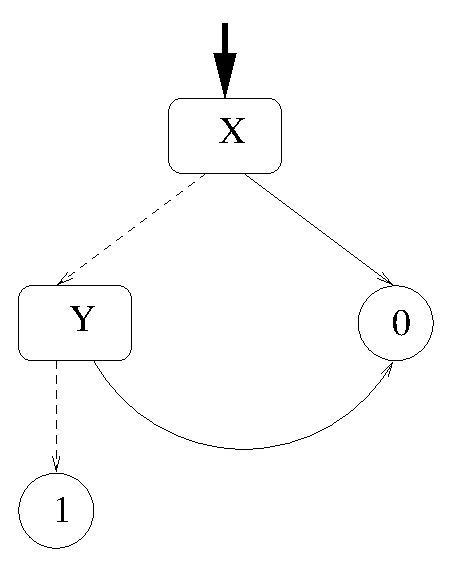
\epsfig{file=bdd2.eps, width=0.23\linewidth}} & & 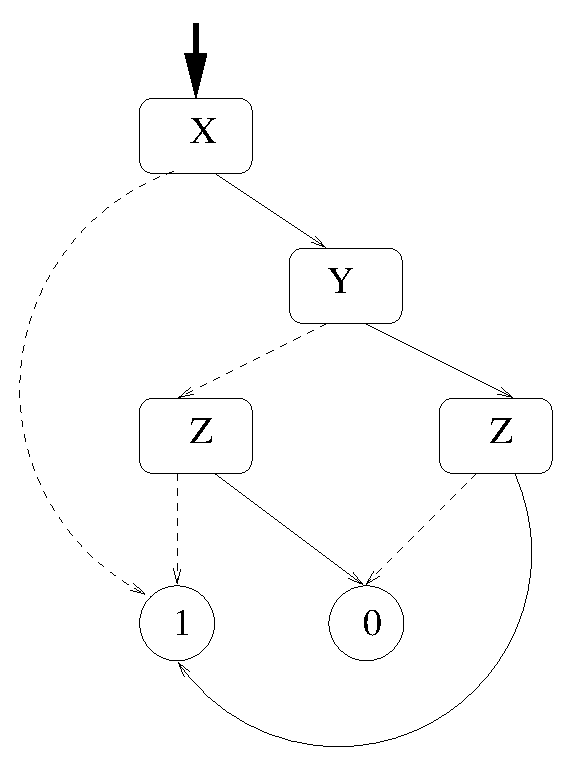
\epsfig{file=bdd1.eps, width=0.3\linewidth}  \\
\etab

\section{Összetett \clpb példa: hibakeresés áramkörben}

Legyen adott egy egybites összeadó áramköri modellje (funkcionális elemekkel
és összeköttetésekkel). Írjunk egy olyan \clpb programot, amely adott
bemenet-kimenet párra megmondja, hogy melyik funkcionális elem működik
hibásan, ha feltételezzük, hogy egyszerre csak egy hibásodik meg!

\begin{center}\insertfig{adder1}{10cm}\end{center}

\begin{minted}{prolog}
fault([F1,F2,F3,F4,F5], [X,Y,Cin], [Sum,Cout]) :-
        sat(
                    card([0-1],[F1,F2,F3,F4,F5]) *
                    (F1 + (U1 =:= X * Cin)) *
                    (F2 + (U2 =:= Y * U3)) *
                    (F3 + (Cout =:= U1 + U2)) *
                    (F4 + (U3 =:= X # Cin)) *
                    (F5 + (Sum =:= Y # U3))
                ).
\end{minted}

Amint látható, a \cd{fault/3} predikátumban semmi mást nem tettünk, mint
specifikáltuk az egyes áramköri elemek működését, valamint a \cd{card}
segítségével megadtuk azt a tényt is, hogy egyszerre legfeljebb egy
áramköri elem hibás. Lássunk néhány példát a \cd{fault} működésére!

\begin{minted}{prolog}
| ?- fault(L, [1,1,0], [1,0]).
                            L = [0,0,0,1,0] ? ;  no
\end{minted}

Itt a \cd{fault} helyesen kikövetkeztette, hogy ilyen bemenet-kimenet
pár esetén csak a 4. funkcionális elem, azaz a programkód alapján
az \cd{X}-re és \cd{Cin}-re kapcsolódó XOR kapu lehet hibás.

\begin{minted}{prolog}
| ?- fault(L, [1,0,1], [0,0]).
                            L = [_A,0,_B,0,0],
                            sat(_A=\=_B) ? ; no
\end{minted}

Itt a \cd{fault} úgy gondolja, hogy vagy az első, vagy a harmadik funkcionális
elem a hibás, ezt a korlát-tárban lévő \cd{sat(_A=\bs=_B)} fejezi ki. Ha
ehelyett látni szeretnénk a két lehetőséget teljesen behelyettesített
változókkal, akkor szükséges a \cd{labeling} használata is:

\begin{minted}{prolog}
| ?- fault(L, [1,0,1], [0,0]), labeling(L).
                            L = [1,0,0,0,0] ? ;
                            L = [0,0,1,0,0] ? ; no
\end{minted}

Végül megkérdezhetjük a \cd{fault}-tól, hogy helyes áramköri működést
feltételezve mik az egyes kimenetekhez rendelhető logikai egyenletek:

\begin{minted}{prolog}
| ?- fault([0,0,0,0,0], [x,y,cin], [Sum,Cout]).
                            sat(Cout=:=x*cin#x*y#y*cin),
                            sat(Sum=:=cin#x#y) ? ; no
\end{minted}

Tekintsünk most egy XOR kaput megvalósító tranzisztoros áramkört, és
valósítsuk meg ennek a verifikációját \clpb programmal!

\begin{center}\insertfig{xor}{8cm}\end{center}

Először leírjuk az npn és pnp tranzisztorok működését \clpb kifejezésekkel:
\begin{minted}{prolog}
n(D, G, S) :-    % Gate => Drain = Source
        sat( G*D =:= G*S).

p(D, G, S) :-    % ~ Gate => Drain = Source
        sat( ~G*D =:= ~G*S).
\end{minted}

Ezek segítségével megfogalmazhatjuk az XOR kapu működését, ha a földelést
0-val, a tápfeszültséget 1-gyel jelöljük:

\begin{minted}{prolog}
xor(A, B, Out) :-
        p(1, A, X),
        n(0, A, X),
        p(B, A, Out),
        n(B, X, Out),
        p(A, B, Out),
        n(X, B, Out).
\end{minted}

Ellenőrizzük, hogy az npn és pnp tranzisztorokra felírt egyenleteink
helyesen működnek-e a gate feszültség ki- és bekapcsolására:

\begin{minted}{prolog}
| ?- n(D, 1, S).                 S = D ?
| ?- n(D, 0, S).                 true ?
| ?- p(D, 0, S).                 S = D ?
| ?- p(D, 1, S).                 true ?
\end{minted}

A fentiek szerint a tranzisztorok logikai felírása helyes, így nem
maradt más hátra, mint hogy ellenőrizzük, hogy az XOR kapu ténylegesen
az XOR függvényt valósítja-e meg:

\begin{minted}{prolog}
| ?- xor(a, b, X).               sat(X=:=a#b) ?
\end{minted}

\section{Aknakereső játék \Clpb -ben}

Az alábbi programkód egy aknakereső játékot valósít meg \clpb programkód
formájában.

\begin{minted}{prolog}
:- use_module([library(clpb),library(lists)]).
\end{minted}
\begin{minted}{prolog}
mine(Rows, Cols, Mines, Bd) :-
        length(Bd, Rows), all_length(Bd, Cols), 
        append_lists(Bd, All),
        sat(card([Mines], All)), play_mine(Bd, []).
\end{minted}
\begin{minted}{prolog}
all_length([], _).
all_length([L|Ls], Len) :- 
        length(L, Len), all_length(Ls, Len).
\end{minted}
\begin{minted}{prolog}
append_lists([], []).
append_lists([L|Ls], Es) :-
        append_lists(Ls, Es0), append(L, Es0, Es).
\end{minted}
\begin{minted}{prolog}
play_mine(Bd, Asked) :- 
        select_field(Bd, Asked, R, C, E), !,
        format('Row ~w, col ~w (m for mine)? ', [R,C]), 
        read(Ans), process_ans(Ans, E, R, C, Bd), 
        play_mine(Bd, [R-C|Asked]).
play_mine(_Bd, _Asked).
\end{minted}
\begin{minted}{prolog}
select_field(Bd, Asked, R, C, E) :-
        nth(R, Bd, L), nth(C, L, E), 
        non_member(R-C, Asked), taut(E, 0), !.
select_field(Bd, Asked, R, C, E) :-
        nth(R, Bd, L), nth(C, L, E), 
        non_member(R-C, Asked), \+ taut(E,1), !.
\end{minted}
\begin{minted}{prolog}
process_ans(m, 1, _, _, _) :- 
        format('Mine!~n', []), !, fail.
process_ans(Ans, 0, R, C, Bd) :-
        integer(Ans), neighbs(n(R, C, Bd), Ns), 
        sat(card([Ans], Ns)).
\end{minted}
\begin{minted}{prolog}
neighbs(RCB, N7) :-
        neighbour(-1,-1, RCB, [], N0), 
        neighbour(-1, 0, RCB, N0, N1),
        neighbour(-1, 1, RCB, N1, N2), 
        neighbour( 0,-1, RCB, N2, N3),
        neighbour( 0, 1, RCB, N3, N4), 
        neighbour( 1,-1, RCB, N4, N5),
        neighbour( 1, 0, RCB, N5, N6), 
        neighbour( 1, 1, RCB, N6, N7).
\end{minted}
\begin{minted}{prolog}
neighbour(ROf, COf, n(R0, C0, Bd), Nbs, [E|Nbs]) :-
        R is R0+ROf, C is C0+COf, 
        nth(R, Bd, Row), nth(C, Row, E), !.
neighbour(_, _, _, Nbs, Nbs).
\end{minted}

A játék belépési pontja a \cd{mine(Rows,Cols,Mines,Bd)} eljárás, amely
egy \cd{Rows} $\times$ \cd{Cols} méretű táblát készít el a \cd{Bd}
listában, és felteszi róla, hogy \cd{Mines} db 1-es van benne.
Ezek után a \cd{play_mine/2} eljáráson keresztül kijelzi, hogy melyik
mező tartalmára kíváncsi, erre a felhasználónak az \cd{m.} karaktersorozattal
kell válaszolnia, ha akna van ott, üres mező esetén pedig meg kell adni, hogy
hány akna található a mező körül. Ha a felhasználó válasza \cd{m.}, akkor a
program szomorúan konstatálja, hogy veszített (\cd{Mine!}), ha viszont egy
szám, akkor a tippelt mező körül lévő mezőkre a \cd{process_ans/5} eljárás
második klózával felveszi a megfelelő számossági korlátot. A következő tipp
kiválasztását a \cd{select_field/5} eljárás végzi, ez mindig egy olyan mezőt
választ ki, amelyről a program egyértelműen tudja, hogy üres (1. klóz), ha ilyet
nem talál, akkor pedig egy olyat, amelyről nem tudja biztosan, hogy aknát tartalmaz
(2. klóz). Egy egyszerű példajáték ($3 \times 3$-as tábla, akna a 2. sor 1. mezőjén
és a 3. sor 3. mezőjén van):

\begin{minted}{prolog}
| ?- mine(3,3,2,Bd).
% az első két lépésben a program csak reménykedik abban, hogy
% nem lép aknára
Row 1, col 1 (m for mine)? 1.
Row 1, col 2 (m for mine)? 1.
% itt a program már rájön, hogy az (1,3) és a (2,3) mező üres
Row 1, col 3 (m for mine)? 0.
% ebből már azt is tudja, hogy a (2,2) mező üres, így viszont
% a (2,1) mezőn akna van
Row 2, col 2 (m for mine)? 2.
% mivel a (2,3) mezőről már előzőleg kikövetkeztette, hogy üres,
% ezért azt is meg meri kérdezni
Row 2, col 3 (m for mine)? 1.
% mivel a (2,2) mező körül már csak 1 akna helyét nem tudjuk,
% de azt is tudjuk, hogy a (2,3) mező körül is 1 akna van, ezért
% a (3,1) mezőn nem lehet akna
Row 3, col 1 (m for mine)? 1.
% így viszont a (3,2) mező is üres
Row 3, col 2 (m for mine)? 2.
Bd = [[0,0,0],[1,0,0],[0,0,1]] ? ;
no
\end{minted}

Vegyük észre, hogy a program inkonzisztens adatok esetén meghiúsulást produkál:

\begin{minted}{prolog}
| ?- mine(3,3,2,Bd).
Row 1, col 1 (m for mine)? 1.
Row 1, col 2 (m for mine)? 1.
Row 1, col 3 (m for mine)? 0.
Row 2, col 2 (m for mine)? 1.
no
\end{minted}

A \clpb mohósága miatt azonban a program egy $20 \times 20$-as aknamezőre már
nagyon hosszú ideig veszi fel a \cd{mine/4}-ben szereplő \cd{sat(card...)}
korlátot (mivel a \cd{card}-ot is ,,polinom'' formára vezeti vissza a listában
szereplő összes változó esetén), ilyenkor a program szinte játszhatatlanul lassú lesz.